\documentclass[10pt,twocolumn,letterpaper]{article}

\usepackage{cvpr}
\usepackage{times}
\usepackage{epsfig}
\usepackage{graphicx}
\usepackage{amsmath}
\usepackage{amssymb}
\usepackage{mathrsfs}
\usepackage{mathtools}
\usepackage{subfigure}


% Include other packages here, before hyperref.

% If you comment hyperref and then uncomment it, you should delete
% egpaper.aux before re-running latex.  (Or just hit 'q' on the first latex
% run, let it finish, and you should be clear).
\usepackage[pagebackref=true,breaklinks=true,letterpaper=true,colorlinks,bookmarks=false]{hyperref}

% \cvprfinalcopy % *** Uncomment this line for the final submission

\def\cvprPaperID{****} % *** Enter the CVPR Paper ID here
\def\httilde{\mbox{\tt\raisebox{-.5ex}{\symbol{126}}}}

% Pages are numbered in submission mode, and unnumbered in camera-ready
\ifcvprfinal\pagestyle{empty}\fi
\begin{document}

%%%%%%%%% TITLE
\title{Learning Bag-of-Multi-Scale-Activations from Deep Convolutional Nets}

\author{First Author\\
Institution1\\
Institution1 address\\
{\tt\small firstauthor@i1.org}
% For a paper whose authors are all at the same institution,
% omit the following lines up until the closing ``}''.
% Additional authors and addresses can be added with ``\and'',
% just like the second author.
% To save space, use either the email address or home page, not both
\and
Second Author\\
Institution2\\
First line of institution2 address\\
{\tt\small secondauthor@i2.org}
}

\maketitle
%\thispagestyle{empty}

%%%%%%%%% ABSTRACT
\begin{abstract}
While Deep Convolutional Neural Network (CNN) encodes multi-scale features with their spatial locations, Bag-of-feature representations are more invariant to spatial translations. In this paper, we propose a CNN architecture transformation schema that extracts multi-scale CNN representations with spatial invariance. By directly channeling multiple average-pooled rectified linear units (ReLU) to the final layer of scoring function, we explicitly learn an augmented model from multi-scale activations. We term this transformation Bag-of-Multi-Scale-Activation (BoMSA) Augmentation. The BoMSA augmented model can be trained from scratch or built upon existing pre-trained models, which makes the augmentation more flexible. BoMSA augmentation is also model-independent and can be easily adapted to existing models. Experimental results show noticeable improvements achieved by incorporating the BoMSA representation on various models in the literature.  

\end{abstract}

%%%%%%%%% BODY TEXT
\section{Introduction}

Deep CNN has shown its versatility in the tasks such object detection[], recognition[], segmentation[], etc. Trained with large number of instances, (such as ImageNet~\cite{ImageNet}), CNN is also an excel candidate for off-the-shelf feature extractions, results in outstanding performance in various recognition tasks~\cite{cnn_baseline}. In the meantime, a considerable amount of effort is spent on how to further improve the performance of CNN. On one hand, many are focus on techniques to efficiently and effective train a CNN. A good initialization need to be carefully selected~\cite{diff_cnn} in the beginning. Data augmentation~\cite{AlexNet} is recommended to improve the model performance as well. Drop-out~\cite{dropout} and momentum~\cite{momentum} are also necessary to prevent over-fitting and obtain superior models. On the other hand, different model components and architectures are proposed. Rectified linear units (ReLU)~\cite{AlexNet} add non-linearity and enrich the model complexity. Different pooling method, such as Distance Transform Pooling~\cite{dist_trans}, is adopted in~\cite{dpm_is_cnn}, allowing local deformations, as in the widely-used deformable part-based model (DPM)~\cite{dpm}. \cite{veryDeep} adopts a small $3\times 3$ receptive field to deepen the model, while maintaining less parameters. A network in network~\cite{nin} is proposed to enhance model discriminability for local patches within the receptive field. The award winning GoogLeNet~\cite{GoogLeNet} uses an \textit{Inception} model that is based on the Hebbian principle~\cite{Hebb}, \ie, neurons that fire together, wire together, the theoretical proof of which is provided by~\cite{dnn_proof} under constraints. 

One question to ponder: is there any model-independent potential that is yet to be discovered. Although allowing local deformation, CNN encodes the the spatial information of multi-scale features. Conversely, by ignoring the spatial location of features, bag-of-feature like techniques~\cite{spatial_pyramid} achieves transformation invariance to some extend. As pointed out in~\cite{Gong14}, combining both type of features results in a better representation for recognition tasks with large variations, such as Scene classification~\cite{SUN397,MIT67}. Using off-the-shelf deep CNN features,~\cite{Gong14} explicitly extracts image patches from three scales and computes the feed-forward CNN activations for each patch. This algorithm is cumbersome due to the compution of multiple patches for one image. Besides, it can only encode the multi-scale features to a certain extend limited by the burden of the post processing, \ie, K-means and Principle Component Analysis (PCA). As a matter of fact, CNN feature is meant to encode multi-scale feature at each convolutional layer. Therefore, only one feed-forward computation is sufficient to capture the activations of multi-scale features for one input image. 

In this paper



as pointed out in~\cite{Gong14}, 

<talk about vanishing gradient problem in deep model>

<spatial-aware deep model vs. bag-of-feature model: talks about multi-scale [Gong14]>

In this paper, present a new model, link ReLU layer for 


Fig. CNN filter visualization at different scale 

%-------------------------------------------------------------------------
%-------------------------------------------------------------------------
\section{Related Work}


%-------------------------------------------------------------------------
%-------------------------------------------------------------------------
\section{Technical Approach}

We seek to discover a model-independent feature representation that can be efficiently computed. This representation should conform the property of \textit{multi-scale} and \textit{orderless} which outperform single-scale representation in scene classification tasks. 

\subsection{Model}

In this work, we consider two models in the literature, namely Caffe and Deep19. Caffe~\cite{Caffe} is a well-known deep learning framework. It has a pre-trained model which follows the landmark ``AlexNet''~\cite{AlexNet} trained with millions of data in the ImageNet dataset~\cite{ImageNet}. This model has 6 conv. layers and 2 fully-connected (FC) layers. Deep19~\cite{veryDeep} uses very small $3\times 3$ receptive fields for the entire net and the deepest model has 19 layers (16 conv. and 3 FC layers). This model registered the state-of-the-art performance in ILSVRC-2014 classification challenge~\cite{ILSVRC14}. 

We intend to demonstrate the consistency and model-independence of our observations and approach. We have conducted experiments on several CNN models and observed similar patterns. Due to limited space, we only provide the analysis of the aforementioned Caffe and Deep19 models as exemplars in the rest of the paper. 

%-------------------------------------------------------------------------
\subsection{Multi-scale Orderless CNN Activation\label{sec:definition}}

We consider the marginal activation of a rectified linear unit (ReLU) as the \textit{orderless} feature response at its corresponding scale. As described in~\cite{ReLU,AlexNet}, ReLU models a neuron's output $r$ as a mapping of its input $x$ with the non-saturating nonlinearity $r(x)=\max (0,x)$. 

Concretely, to compute the proposed representation, let $\alpha_i$ of dimension $w\times h\times k$ be the output of ReLU at $i$-th layer ($w=h$ in most CNN models). Each $w\times h$ is the convolutional response map of one of the $k$ filters. It carries the spatial activation information at the current scale. Thus, the \textit{orderless} response, $f_i$, at each scale can be computed by sum-pooling the first two dimension of $\alpha_i$, resulting in a $k$-dimensional vector, \ie,

\begin{equation}
f_i=\sum_w \sum_h \alpha_i
\end{equation}

We are motivated to choose the output of the ReLU layer due to the nonlinearity it introduces to the CNN architecture, which boosts the discriminative power of the model. To further provide statistical evidences for the argument, we conduct classification experiments on MIT Indoor Scene (MIT67) dataset~\cite{MIT67} using both Caffe and Deep19 models. We consider the orderless response, $f_i$, from each layer as different features; one-vs-all linear SVMs are then trained and the classification accuracy is reported in Fig.~\ref{fig:layer_MIT67}. The detailed experimental setups for both Caffe and Deep19 models are similar to the ones described in Sec.~\ref{sec:exp}. As seen in Fig.~\ref{fig:layer_MIT67}, in general, the discriminativeness of the model increases as the layer becomes higher. More importantly, we observe significant improvement resulting from each ReLU layer. These observations not only inform us that the CNN model owes its performance boost to the nonlinearity of the ReLU layer, but also motivate us to leverage multiple ReLU layer responses to enrich the discriminative ability of the model. 

\begin{figure}[htbp]
\centering
	\subfigure[Caffe]{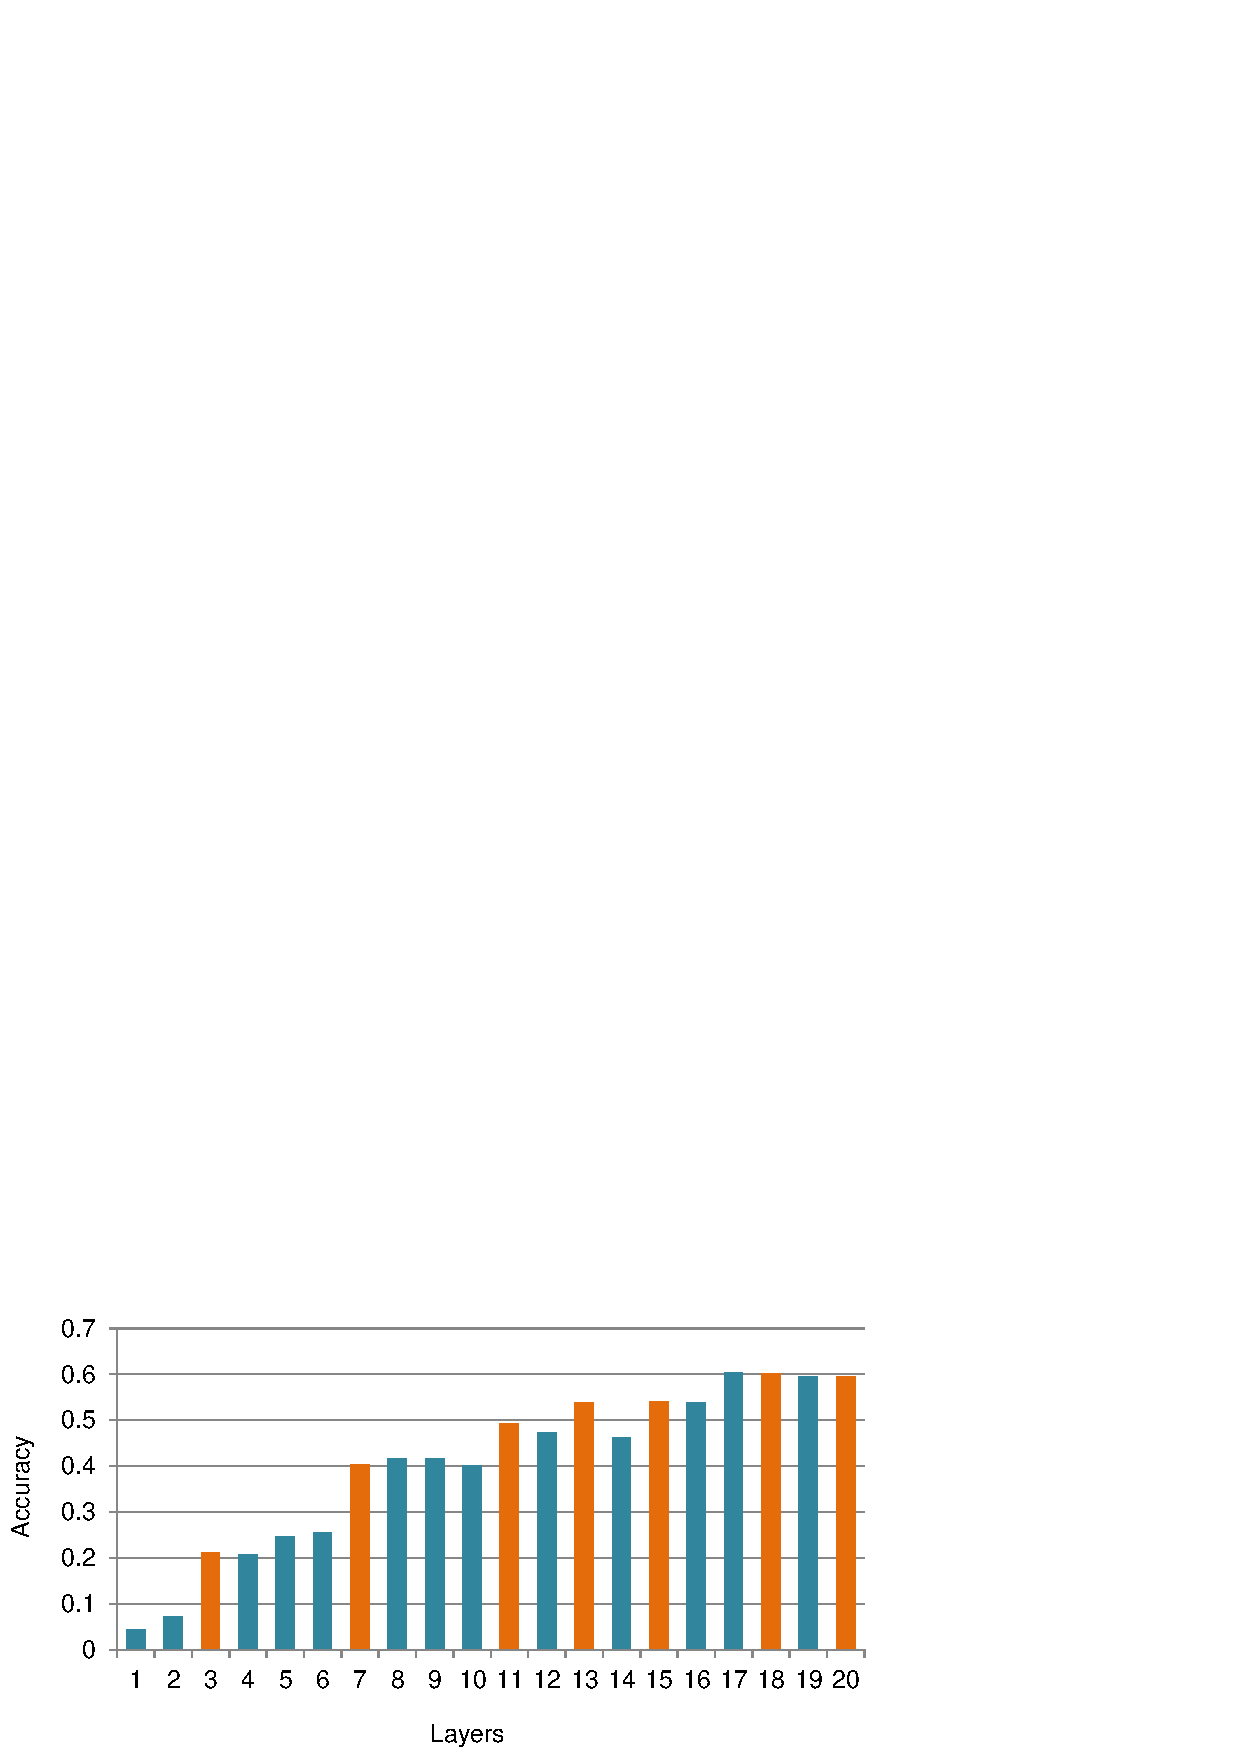
\includegraphics[width=\columnwidth]{fig_layer_caffe.png}\label{fig:layer_caffe}}
	\subfigure[Deep19]{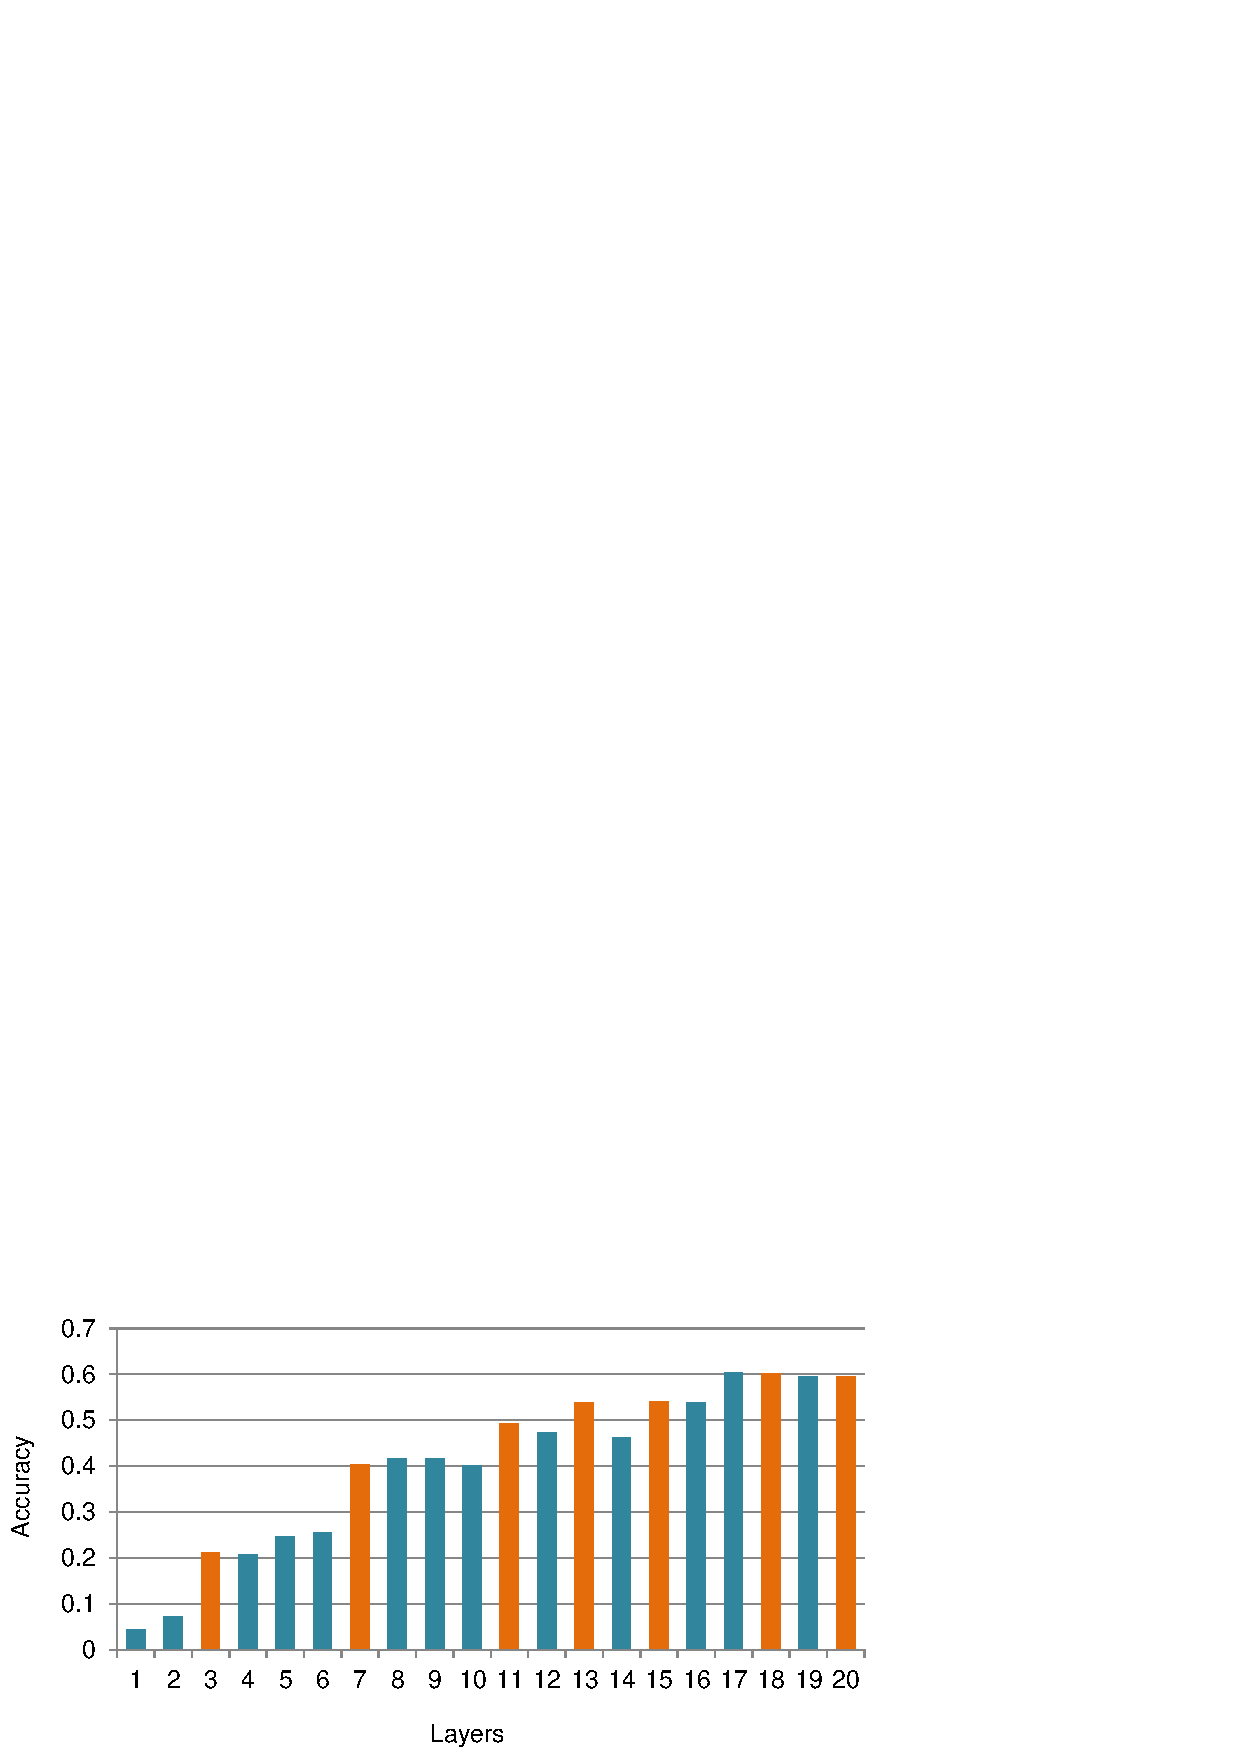
\includegraphics[width=\columnwidth]{fig_layer_caffe.png}\label{fig:layer_deep19}}
\caption{The classification accuracy on MIT67~\cite{MIT67} using the marginal activation of each layer. The color alternation indicates change of convolutional layers. The solid color fill represents the output of the ReLU layer. There are 7 ReLU layer for the Caffe model and 18 for Deep19. A significant performance improvement is observed at each ReLU layer compared with its previous layer, especially at the early convolutional layers.}

\label{fig:layer_MIT67}
\end{figure}


%-------------------------------------------------------------------------
\subsection{The Feature Selection from Activation Layer}

Since different CNN layer models image patterns at various scales, the first question to ask is that ``Does combining activations at all scales help to extract a better feature''?  To address this question, we carried out another experiments on the MIT67 data~\cite{MIT67}. In the literature when CNN is used for feature extraction, the response of the first fully connected layer is usually selected. Our previous analysis in Fig.~\ref{fig:layer_MIT67} also demonstrates the discriminative power of high-level CNN layer. Thus, in this experiment, we start from the $f$ of the last ReLU layer and greedily concatenate the marginal responses from previous ReLU layer. The rest of the experimental setups are the same as in Sec.~\ref{sec:definition} and Sec.~\ref{sec:exp}, \ie, 67-way one-vs-all linear SVM classifiers are trained every time we add one more layer. Since we keep on concatenating the $f$s to our feature, the feature dimension is monotonically increasing. As the results shown in Fig.~\ref{fig:add_back}, the performance increase in the beginning by adding mid-level features to enrich the model discriminativeness. However, including some low level responses to the feature actually hurts the performance, \ie, layer 7 and 3 in Fig.~\ref{fig:add_back_caffe}. We believe it demonstrates the benefit of incorporating more discriminative mid-level and high-level features of CNN (\ie, \textit{parts} and \textit{objects}), but not necessarily the low-level features, such as \textit{corner} or \textit{edge}. 

\begin{figure}[htbp]
\centering
	\subfigure[Caffe]{\includegraphics[width=.49\columnwidth]{fig_add_back_caffe.png}\label{fig:add_back_caffe}}
	\subfigure[Deep19]{\includegraphics[width=.49\columnwidth]{fig_add_back_caffe.png}\label{fig:add_back_deep19}}
\caption{The performance trend when incorporating more $f$ from the ReLU layer. The keyword ``all'' means previous $f$s been included as feature. A performance drop is observed when incorporating low level marginal responses.}

\label{fig:add_back}
\end{figure}


A more systematic way to select the layers to incorporate as feature is feature forward selection, \ie, greedily add the layer in the ReLU pool which results in the best performance boost in an iterative manner. As seen in Fig.~\ref{fig:forward_select_caffe}, the optimal results of this greedy approach is congruent with the previous results in Fig.~\ref{fig:add_back_caffe}, which rejects the low-level features. Similarly for the Deep19 model in Fig.~\ref{fig:forward_select_deep19}, although the feature pool is large (18 ReLU layers), the optimal greedy results only selects the mid- or high-level filter responses. 

\begin{figure}[htbp]
\centering
	\subfigure[Caffe]{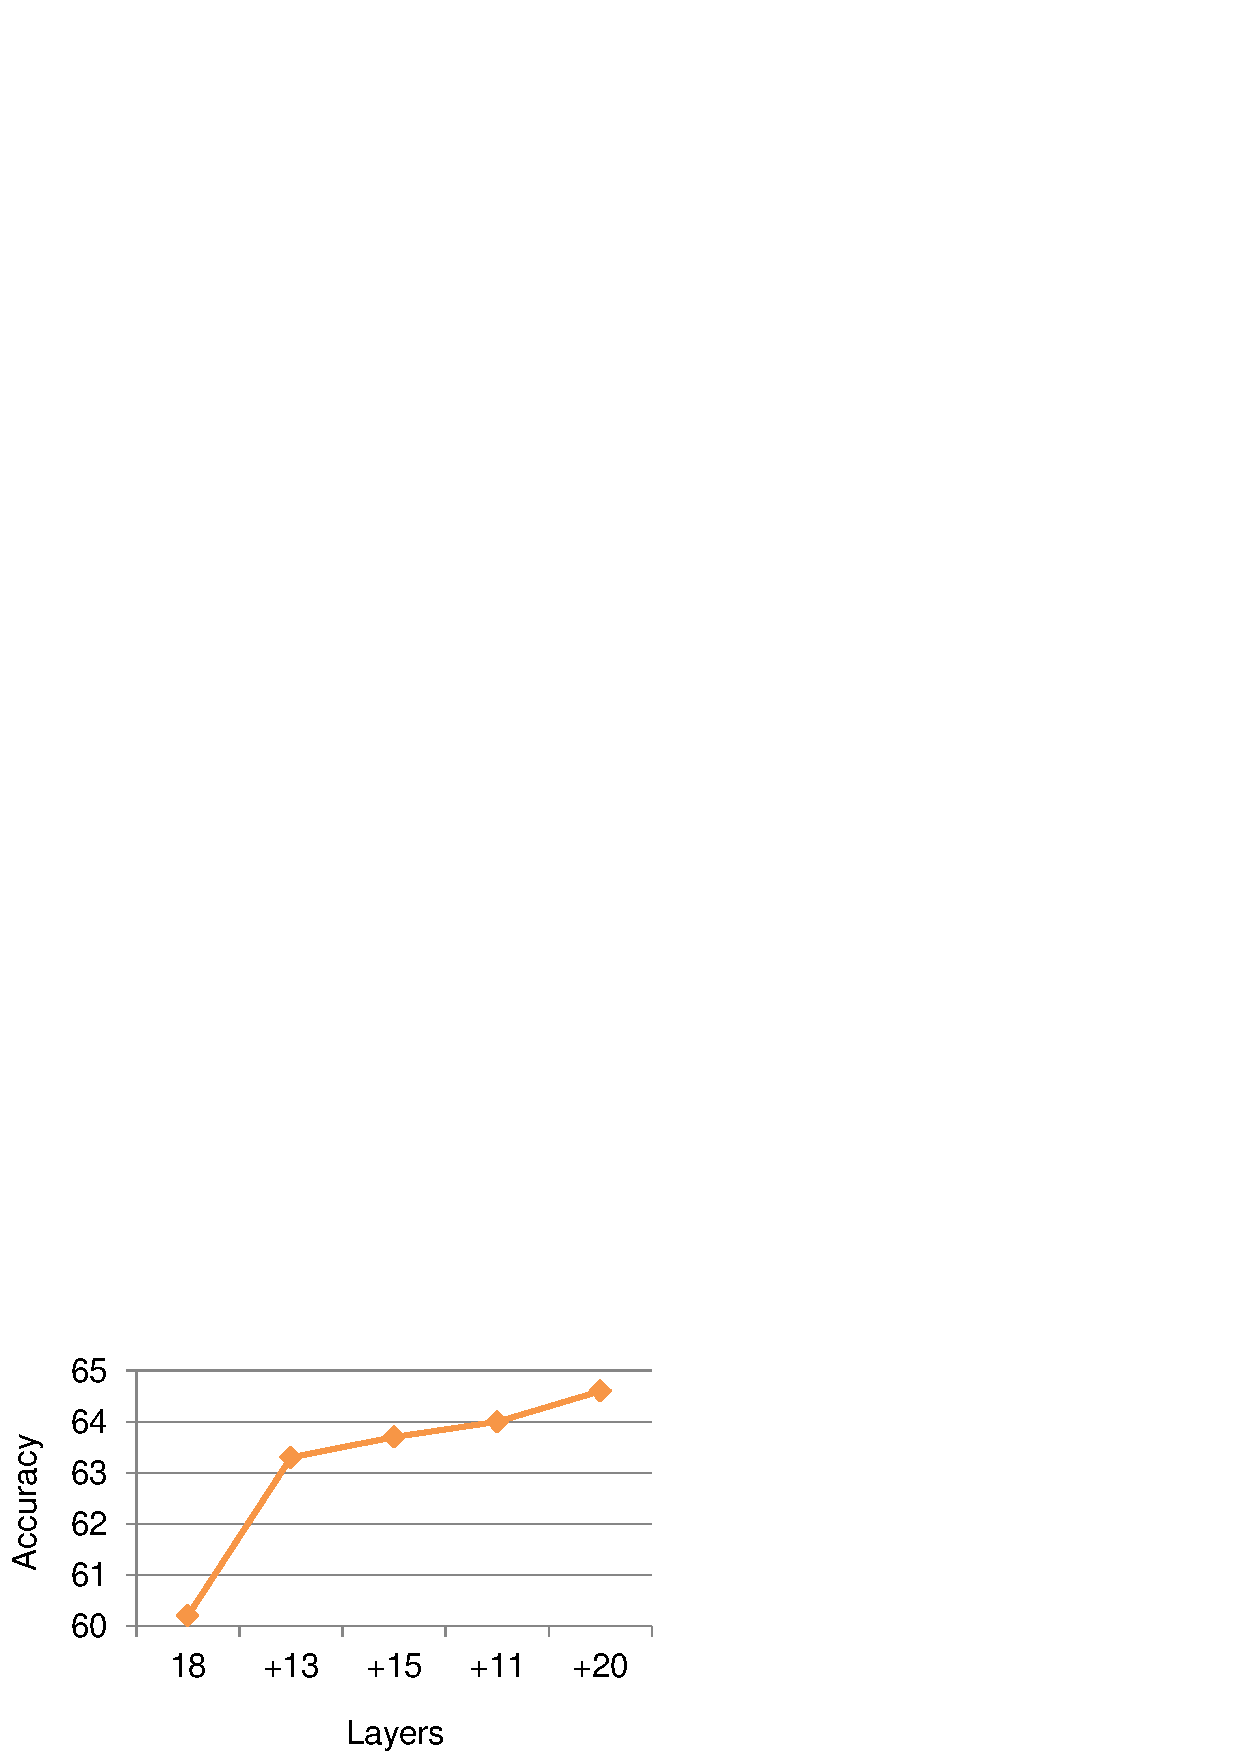
\includegraphics[width=.49\columnwidth]{fig_forward_select_caffe.png}\label{fig:forward_select_caffe}}
	\subfigure[Deep19]{\includegraphics[width=.49\columnwidth]{fig_forward_select_deep19.png}\label{fig:forward_select_deep19}}
\caption{The performance trend when using forward selection to incorporate $f$s from the ReLU layer. }

\label{fig:forward_select}
\end{figure}

By incorporating marginal responses from multiple layers, we have achieved \textit{multi-scale orderless} feature extraction. We term this feature ``MOFeat''. We should point out that for the latter analysis and experiments on other datasets, we opt to use the same feature selected by the forward selection algorithm on MIT67 data. An consistent performance boost demonstrates the data-independence of the proposed feature representation. 

\subsubsection{Discussions}

Though inspired by~\cite{Gong14}, our computation of the \textit{multi-scale orderless} feature is completely different from them. In~\cite{Gong14}, local patches at three scales are first extracted (roughly 50 patches per image in their setting); each patch is then feed to the entire CNN and the activations of the first fully connected layer (4096-dimension) are used for post processing, \ie, K-means + VLAD pooling. 

Our approach has several advantages over~\cite{Gong14}:
\begin{enumerate}
\item \cite{Gong14} computes multiple feed-forward on a single image due to multiple patches. The computation of convolution is the bottleneck for this procedure. In our implementation, only one feed-forward computation is needed for one image and the activation is available at each scale.
\item \cite{Gong14} uses K-means clustering algorithm in the VLAD pooling, which can result in inconsistent result due to random initialization. 
\item \cite{Gong14} conducts two steps of PCA (first PCA to reduce $4096$-dimensional activation to $500$-dimension, and second PCA to reduce $50,000$-dimensional VLAD pooled feature to $4096$-dimension). 
\item the feature extraction procedure in~\cite{Gong14} takes more than 20 seconds for one test image while ours only take less than 1 second. 
\end{enumerate} 

Overall, the implementation of \textit{multi-scale orderless} feature in~\cite{Gong14} is not only inefficient but also prone to over-fitting due to a number of hyper-parameter tuning. On the contrary, our implementation is easy to compute and little parameter tuning is needed. 

%-------------------------------------------------------------------------
\subsection{The Analysis of Invariance}

Besides the insight on visualizing deep CNN features,~\cite{visual_cnn} provides transformation invariance analysis of their model on several images. This is done by comparing the feature vector distance between the original and transformed images. Realizing that several examples do not necessarily represents the overall statistics,~\cite{Gong14} improve the invariance analysis by experiments on the SUN397 scene database~\cite{SUN397}. Unfortunately, only the results on 4 categories are provided in their paper. The performance for the entire dataset is still unknown

%and the invariance definition is difficult to quantify. 
%\textbf{[We should provide some metric to measure the invariance as one of the contribution.]}

To cope with the aforementioned gap and analyze the invariance of our representation, we carried out experiments on the entire MIT Indoor dataset~\cite{MIT67} and report the average performance. We intend to compare the tolerance of the proposed multi-scale MOFeat compared with single-scale CNN features. Concretely, the single-scale CNN feature in comparison is the activation of CNN model which achieves best classification performance (not necessarily the output of the first FC layer). We first trained $67$-way one-vs-all linear SVM classifiers for all $67$ classes using features extracted from the original images. During test phase, four transformations are considered for the analysis, \ie, translation, scaling, flipping, and rotation. Fig.~\ref{fig:invar_eg} illustrates all the transformations and their corresponding parameters, which are similar to the ones in~\cite{Gong14}. After applying the transformations to test images, features are extracted for the proposed MOFeat and single-scale feature. The classification is conducted using the trained SVMs, and the accuracy is shown in Fig.~\ref{fig:invar_rst}. Each data point is the performance of the entire test data. As seen in Fg.~\ref{fig:invar_rst}, the transformations almost always hurt the performance except for horizontal flip. This observation is similar to the one in~\cite{Gong14}. We also see that multi-scale feature, MOFeat, consistently out-performs the single-scale feature under every degree of all transformations. As far as the invariance is concerned, we observe the same level of performance decrease, if not more, for MOFeat compared with single-scale. This means that both features have the same level of tolerance to transformations. This immediately suggest that ``training jittering'', \ie, including transformations in the training data, will improve the performance. Since ``training jittering'' is conducted during the training of CNN model for classification~\cite{veryDeep}, it is interesting that the observation of our invariance analysis shows that when using CNN for feature extraction, it is beneficial to perform another round of ``training jittering'' to train the classifiers. 


\begin{figure}[htbp]
\centering
	\subfigure[v-translation]{\includegraphics[width=.49\columnwidth]{invar/v.png}\label{fig:inv_v}}
	\subfigure[scaling]{\includegraphics[width=.49\columnwidth]{invar/s.png}\label{fig:inv_s}}
	\subfigure[h-translation]{\includegraphics[width=.49\columnwidth]{invar/h.png}\label{fig:inv_h}}
	\subfigure[flipping]{\includegraphics[width=.49\columnwidth]{invar/f.png}\label{fig:inv_f}}
	\subfigure[rotation]{\includegraphics[width=.49\columnwidth]{invar/r.png}\label{fig:inv_r}}

\caption{The classification accuracy of various transformations on test images in MIT67 data~\cite{MIT67}. The legends shown in Fig.~\ref{fig:inv_v} is the same in the other four figures.}

\label{fig:invar_rst}
\end{figure}

%-------------------------------------------------------------------------
%-------------------------------------------------------------------------
\section{Experimental Results\label{sec:exp}}

In this section, we carried out experiments on benchmark dataset, SUN397~\cite{SUN397}, MIT67~\cite{MIT67}, and Scene15~\cite{Scene15} to demonstrate the consistency of our approach. We should stress that our MOFeat representation is learned on MIT67 and applied to all the experiments.

\section{Experiment Setup}

We follow the standard image pre-processing steps in the literature~\cite{AlexNet,Caffe,veryDeep}. Since both Caffe~\cite{Caffe} and Deep19 models~\cite{veryDeep} have a fixed input size of $224\times 224$, we first resize the image such that the smaller side matches $224$, and then crop an $224\times 224$ patch from the center. The mean RGB value of each model learned on ImageNet~\cite{ImageNet} is then subtracted.  


consistent performance improvement on all scene dataset

1. SUN397

2. MIT67

3. Scene15

%-------------------------------------------------------------------------
%-------------------------------------------------------------------------
\section{Conclusion}




{\small
\bibliographystyle{ieee}
\bibliography{mobib}
}

\end{document}
